\subsection{Introdução}

A validação da aplicação desenvolvida constitui uma etapa essencial para demonstrar a fiabilidade dos algoritmos de dimensionamento implementados para vigas, pilares e sapatas isoladas segundo Eurocódigo EC2 A formulação teórica dos modelos de cálculo e dos critérios normativos foi previamente estabelecida nos Capítulos 3 e 4, pelo que o presente capítulo se centra na verificação prática das entradas, do processamento interno e das saídas produzidas pela aplicação.

A estratégia adotada combina dois níveis complementares de validação. Por um lado, recorrem-se a casos de teste automatizados, integrados no ambiente de desenvolvimento, com o objetivo de garantir a consistência do código ao longo da evolução do sistema. Por outro lado, procede-se à comparação detalhada entre os resultados da aplicação e exemplos resolvidos de obras de referência, designadamente Goodchild et al. \cite{Goodchild} e Mosley et al. \cite{Mosley}, permitindo aferir a coerência estrutural e normativa dos resultados obtidos.

\subsection{Metodologia de Teste}

A validação computacional foi estruturada com base em testes unitários automatizados, implementados no ambiente Django. Esta abordagem permite verificar, de forma repetível e objetiva, se as funções responsáveis pelo dimensionamento dos diferentes elementos retornam resultados compatíveis com os valores esperados para um conjunto conhecido de dados de entrada.

Cada teste define previamente a geometria, os materiais, os carregamentos e os parâmetros regulamentares do elemento estrutural a analisar, executando depois o serviço de cálculo correspondente. Os resultados produzidos são comparados com valores de referência, obtidos por resolução manual ou extraídos de exemplos académicos reconhecidos. Deste modo, assegura-se não apenas a correção matemática das rotinas implementadas, mas também a sua estabilidade perante futuras alterações ao código.

Para complementar esta verificação automática, foram selecionados três casos de estudo representativos: um caso de dimensionamento à flexão simples de uma viga, um caso de dimensionamento de um pilar sujeito a flexão composta com verificação de esbelteza, e um caso de dimensionamento de uma sapata isolada sujeita a carga centrada. Estes três exemplos permitem cobrir diferentes mecanismos resistentes e diferentes tipos de verificação previstos no Eurocódigo 2.

\subsection{Casos de Teste e Resultados}

\subsubsection{Validação da viga}

A validação do módulo de vigas foi realizada com base num caso de flexão simples em secção retangular, comparando a solução produzida pela aplicação com a resolução de referência apresentada por Goodchild et al. \cite{Goodchild} e com o relatório interno da aplicação. O objetivo principal desta validação é confirmar a correção do cálculo da altura útil, do momento reduzido, da área de armadura necessária e da solução construtiva final adotada.

\paragraph{Enunciado do caso de validação}

Considere-se a secção de apoio intermédio de uma viga contínua de betão armado, de secção retangular com largura \(b = 300\ \text{mm}\) e altura total \(h = 450\ \text{mm}\). O momento fletor de cálculo atuante é \(M_{Ed} = 193.8\ \text{kNm}\). Os materiais adotados são betão C30/37 \((f_{ck}=30\ \text{MPa})\), aço A500 \((f_{yk}=500\ \text{MPa})\) e recobrimento nominal \(c_{nom}=35\ \text{mm}\). A Figura~\ref{fig:viga_validacao} apresenta a geometria simplificada da secção analisada.

\begin{figure}[H]
\centering
\begin{tikzpicture}[>=Stealth, scale=1.0]
\draw[thick, fill=gray!15] (0,0) rectangle (3,4.5);
\draw[<->] (0,-0.5) -- (3,-0.5) node[midway, below] {$300\ \text{mm}$};
\draw[<->] (-0.5,0) -- (-0.5,4.5) node[midway, left] {$450\ \text{mm}$};
\end{tikzpicture}
\caption{Secção transversal da viga considerada na validação.}
\label{fig:viga_validacao}
\end{figure}

\paragraph{Resolução segundo Goodchild et al.}

Segundo o Exemplo 4.1 de Goodchild et al.~\cite{Goodchild}, o procedimento manual recorre inicialmente a simplificações para avaliar as dimensões exigidas:

Altura útil é inicialmente estimada admitindo estribos de \(10\ \text{mm}\) e armadura longitudinal de \(25\ \text{mm}\), obtendo-se:
\begin{equation}
d = 450 - 35 - 10 - \frac{25}{2} = 392\ \text{mm}
\end{equation}

O coeficiente reduzido de momento resulta:
\begin{equation}
K = \frac{M_{Ed}}{b d^2 f_{ck}}
= \frac{193.8 \times 10^6}{300 \times 392^2 \times 30}
= 0.142
\end{equation}

Como o valor calculado se mantém dentro do domínio de flexão simples, a secção pode ser tratada sem necessidade de armadura de compressão. Admitindo um braço interno aproximado \(z \approx 0.864d\), obtém-se:
\begin{equation}
z \approx 0.864 \times 392 = 338\ \text{mm}
\end{equation}

A área de armadura necessária é:
\begin{equation}
A_{s,req} =
\frac{M_{Ed}}{f_{yd} z}
=
\frac{193.8 \times 10^6}{(500/1.15)\times 338}
= 1319\ \text{mm}^2
= 13.19\ \text{cm}^2
\end{equation}

Garantindo a verificação das disposições mínimas do Eurocódigo, resulta:
\begin{equation}
    A_{s,min} = \max\left[ 0{,}26 \left( \frac{f_{ctm}}{f_{yk}} \right) b_t \cdot d;\, 0{,}0013 \cdot b_t \cdot d \right] = 177\ \text{mm}^2 = 1{,}77\ \text{cm}^2
\end{equation}

A solução adotada na referência é \(3\phi25\), correspondente a \(14.73\ \text{cm}^2\), valor superior ao requerido.

\paragraph{Resolução pela aplicação desenvolvida}

Na aplicação, o cálculo é realizado de forma iterativa. Numa primeira iteração, assume-se \(\phi_{est}=8\ \text{mm}\) para os estribos e \(\phi_{long}=16\ \text{mm}\), resultando:
\begin{equation}
d_1 = 450 - 35 - 8 - \frac{16}{2} = 399.0\ \text{mm}
\end{equation}

Com este valor, o memento reduzido inicial é:
\begin{equation}
\mu_1 =
\frac{193800}{0.3 \times 0.399^2 \times 20\times 10^6}
= 0.203
\end{equation}

Como a solução de varão único apontada na primeira aproximação difere do diâmetro inicialmente assumido, o algoritmo executa uma segunda iteração com \(\phi = 25\ \text{mm}\), recalculando a altura útil:
\begin{equation}
d_2 = 450 - 35 - 8 - \frac{25}{2} = 394.5\ \text{mm}
\end{equation}

O momento reduzido final passa a:
\begin{equation}
\mu_2 =
\frac{193800}{0.3 \times 0.395^2 \times 20\times 10^6}
= 0.208
\end{equation}

Com base neste valor, a aplicação determina:
\begin{equation}
\xi = \frac{1-\sqrt{1-2\mu}}{0.8} = 0.294
\end{equation}
\begin{equation}
z = d(1-0.5\times 0.8 \times 0.294) = 0.348\ \text{m}
\end{equation}
\begin{equation}
A_{s,req} =
\frac{193800}{0.348 \times 434.78\times 10^6}
= 12.80\ \text{cm}^2
\end{equation}

A solução final mais económica encontrada pelo algoritmo é:
\begin{equation}
2\phi10 + 4\phi20
\end{equation}
com área total:
\begin{equation}
A_{s,prov} = 14.14\ \text{cm}^2
\end{equation}

A armadura mínima calculada pela aplicação é \(1.78\ \text{cm}^2\), pelo que a solução adotada satisfaz confortavelmente a exigência regulamentar. Além disso, a aplicação acrescenta uma armadura superior construtiva \(2\phi10\), destinada ao apoio e amarração dos estribos, sem participação no momento resistente principal.

\begin{table}[H]
\centering
\caption{Comparação entre a referência e a aplicação para a viga.}
\label{tab:comp_viga}
\renewcommand{\arraystretch}{1.2}
\begin{tabular}{lcc}
\toprule
\textbf{Parâmetro} & \textbf{Goodchild et al.} & \textbf{Aplicação} \\
\midrule
Secção [mm] & \(300 \times 450\) & \(300 \times 450\) \\
\(M_{Ed}\) [kNm] & 193.8 & 193.8 \\
Altura útil \(d\) [mm] & 392 & 394.5 \\
Momento reduzido & 0.142 & 0.208 \\
\(A_{s,req}\) [cm\(^2\)] & 13.19 & 12.80 \\
Armadura adotada & \(3\phi25\) & \(2\phi10 + 4\phi20\) \\
\(A_{s,prov}\) [cm\(^2\)] & 14.73 & 14.14 \\
\bottomrule
\end{tabular}
\end{table}

\paragraph{Comparação dos resultados}
Os resultados revelam uma concordância muito satisfatória entre ambas as abordagens. A diferença principal resulta do facto de a aplicação recalcular explicitamente a altura útil e o braço mecânico com base na solução efetivamente adotada, enquanto a resolução de referência usa simplificações de pré-dimensionamento mais diretas.
Ainda assim, a área de armadura final obtida pela aplicação mantém-se muito próxima da referência e confirma a consistência do algoritmo implementado.

\subsubsection{Validação do pilar}

A validação do módulo de pilares foi realizada com base no Exemplo 5.1 de Goodchild et al. \cite{Goodchild}, correspondente a um pilar de bordo sujeito a esforço axial elevado e momentos de extremidade opostos. Este caso é particularmente relevante porque permite testar a verificação de esbelteza, a consideração dos efeitos de segunda ordem e o dimensionamento da armadura longitudinal em flexão composta reta.

\paragraph{Enunciado do caso de validação}

Considere-se um pilar com secção quadrada \(300 \times 300\ \text{mm}\), comprimento real \(l = 3.75\ \text{m}\), ligação encastrada no topo e articulada na base. O esforço axial de cálculo é \(N_{Ed}=1620\ \text{kN}\) e o momento fletor de primeira ordem considerado na aplicação é \(M_{0Ed}=51.4\ \text{kNm}\). Os materiais adotados são betão C30/37 \((f_{ck}=30\ \text{MPa})\), aço A500 \((f_{yk}=500\ \text{MPa})\) e recobrimento nominal \(c_{nom}=25\ \text{mm}\). A Figura~\ref{fig:pilar_validacao} representa o esquema simplificado do elemento.

\begin{figure}[H]
\centering
\begin{tikzpicture}[>=Stealth, scale=1.0]
\draw[thick] (0,0) rectangle (1.5,6);
\draw[thick] (-0.5,6) -- (2.0,6);
\draw[thick] (0.75,0) circle (0.12);
\draw[->, ultra thick] (0.75,7.2) -- (0.75,6.2);
\draw[->, thick] (1.4, 6.5) arc (0:180:0.65);
\node at (2.6, 7.0) {$M_{0Ed} = 51.4\ \text{kNm}$};
\draw[<->] (-1.5,0) -- (-1.5,6) node[midway, left] {$3.75\ \text{m}$};
\node at (0.75,7.5) {$N_{Ed} = 1620\ \text{kN}$};
\node at (3.4,5.2) {Topo: encastrado};
\node at (3.2,0.4) {Base: articulada};
\node at (0.75,-0.5) {$300\ \text{mm}$};
\end{tikzpicture}
\caption{Esquema do pilar considerado na validação.}
\label{fig:pilar_validacao}
\end{figure}

\paragraph{Resolução segundo Goodchild et al.}

No exemplo de referência, o fator de comprimento eficaz é \(\beta = 0.85\), pelo que:
\begin{equation}
l_0 = \beta \cdot l = 0.85 \times 3750 = 3187.5\ \text{mm}
\end{equation}

O raio de giração para a secção quadrada é:
\begin{equation}
i = \frac{h}{\sqrt{12}} = \frac{300}{\sqrt{12}} = 86.6\ \text{mm}
\end{equation}

A esbelteza resulta:
\begin{equation}
\lambda = \frac{l_0}{i} = \frac{3187.5}{86.6} = 36.8
\end{equation}

Segundo a formulação adotada por Goodchild et al., com \(A=0.7\), \(B=1.1\), \(C=2.7\) e \(n=1.06\), a esbelteza limite é:
\begin{equation}
\lambda_{lim}= \frac{20 \cdot A \cdot B \cdot C}{\sqrt{n}} = \frac{20 \cdot 0.7 \cdot 1.1 \cdot 2.7}{\sqrt{1.06}} = 40.4
\end{equation}

Como \(\lambda < \lambda_{lim}\), o pilar é classificado como não esbelto na referência, pelo que não são considerados efeitos adicionais de segunda ordem. O momento de dimensionamento permanece \(M_{Ed} = 51.4\ \text{kNm}\) e a armadura longitudinal adotada na referência é \(4H25\), correspondente a \(A_{s} = 1964\ \text{mm}^2 = 19.64\ \text{cm}^2\).

\paragraph{Resolução pela aplicação}

Na aplicação, o fator de comprimento eficaz é igualmente \(\beta=0.85\), pelo que:
\begin{equation}
l_0 = 0.85 \times 3.75 = 3.188\ \text{m}
\end{equation}

As resistências de cálculo são:
\begin{equation}
f_{cd} = \frac{30}{1.5} = 20.00\ \text{MPa}
\end{equation}
\begin{equation}
f_{yd} = \frac{500}{1.15} = 434.78\ \text{MPa}
\end{equation}

O valor de esbelteza é:
\begin{equation}
\lambda = \frac{3188}{86.6} = 36.81
\end{equation}

A aplicação usa:
\begin{equation}
n = \frac{N_{Ed}}{A_c f_{cd}} = 0.900
\end{equation}
\begin{equation}
A = 1.0,\quad B = 1.1,\quad C = 0.7
\end{equation}

Logo:
\begin{equation}
\lambda_{lim} = \frac{20 \cdot A \cdot B \cdot C}{\sqrt{n}} = 16.23
\end{equation}

Como \(\lambda = 36.81 > 16.23\), a aplicação classifica o elemento como esbelto e ativa o cálculo de segunda ordem pelo método da curvatura nominal.

A curvatura inicial é:
\begin{equation}
\frac{1}{r_0} = \frac{\varepsilon_{yd}}{0.45d} = 0.00001865\ \text{mm}^{-1}
\end{equation}

Com \(\omega \approx 0.090\), \(K_r=0.275\), \(\beta=0.255\) e \(K_\phi=1.000\), resulta:
\begin{equation}
\frac{1}{r} = 0.275 \times 1.000 \times 0.00001865 = 0.00000514\ \text{mm}^{-1}
\end{equation}

A excentricidade de segunda ordem é:
\begin{equation}
e_2 = \frac{1}{r}\frac{l_0^2}{10} = 5.2\ \text{mm}
\end{equation}

O momento adicional é:
\begin{equation}
M_2 = N_{Ed}\times e_2 = 1620 \times 0.0052 = 8.45\ \text{kNm}
\end{equation}

Assim, o momento total de dimensionamento torna-se:
\begin{equation}
M_{Ed,total} = 51.40 + 8.45 = 59.85\ \text{kNm}
\end{equation}

Quanto à armadura, a aplicação calcula:
\begin{equation}
A_{s,min} = \max\left(0.10\frac{N_{Ed}}{f_{yd}},\ 0.002A_c\right)=3.73\ \text{cm}^2
\end{equation}
\begin{equation}
A_{s,req} = 7.75\ \text{cm}^2
\end{equation}
\begin{equation}
A_{s,max}=36.00\ \text{cm}^2
\end{equation}

A solução construtiva ótima é:
\begin{equation}
4\phi16
\end{equation}
com área fornecida:
\begin{equation}
A_{s,prov} = 8.04\ \text{cm}^2
\end{equation}

\begin{table}[H]
\centering
\caption{Comparação entre a referência e a aplicação para o pilar.}
\label{tab:comp_pilar}
\renewcommand{\arraystretch}{1.2}
\begin{tabular}{lcc}
\toprule
\textbf{Parâmetro} & \textbf{Goodchild et al.} & \textbf{Aplicação} \\
\midrule
Secção [mm] & \(300 \times 300\) & \(300 \times 300\) \\
\(M_{Ed}\) [kNm] & 51.4 & 51.4 \\
\(V_{Ed}\) [kNm] & 1620 & 1620 \\
Comprimento eficaz \(l_0\) [m] & 3.1875 & 3.19 \\
Esbelteza \(\lambda\) & 36.8 & 36.81 \\
Esbelteza limite \(\lambda_{lim}\) & 40.4 & 16.23 \\
Classificação & Não esbelto & Esbelto \\
Momento de cálculo [kNm] & 51.4 & 59.85 \\
Armadura adotada & \(4H25\) & \(4\phi16\) \\
Área de aço [cm\(^2\)] & 19.64 & 8.04 \\
\bottomrule
\end{tabular}
\end{table}

\paragraph{Comparação dos resultados}
As diferenças observadas decorrem essencialmente dos parâmetros normativos adotados. Enquanto a referência segue o enquadramento do Anexo Nacional britânico, com \(\alpha_{cc}=0.85\) e um valor elevado de \(C\) para dupla curvatura, a aplicação usa diretamente os valores base do EC2, com \(\alpha_{cc}=1.0\) e \(C=0.7\), conduzindo a uma verificação mais conservadora da esbelteza. Ainda assim, o comportamento global do algoritmo é coerente, e o caso comprova que a aplicação trata corretamente a transição entre pilares não esbeltos e pilares esbeltos, bem como o cálculo dos efeitos de segunda ordem.

\subsubsection{Validação da sapata}

A validação do módulo de sapatas isoladas foi realizada com base no Exemplo 10.1 de Mosley et al \cite{Mosley}, correspondente ao dimensionamento de uma sapata centrada para um pilar quadrado. Este caso permite avaliar a coerência do algoritmo em três etapas fundamentais: o dimensionamento geotécnico em serviço, a verificação ao punçoamento em estado limite último e o dimensionamento da armadura inferior de flexão.

\paragraph{Enunciado do caso de validação}

Considere-se uma sapata isolada que suporta um pilar quadrado com secção \(400 \times 400\ \text{mm}\). As ações características aplicadas são \(G_k = 1000\ \text{kN}\) e \(Q_k = 350\ \text{kN}\). A tensão admissível do terreno é \(\sigma_{adm}=200\ \text{kN/m}^2\). Os materiais considerados são betão C30/37 \((f_{ck}=30\ \text{MPa})\), aço A500 \((f_{yk}=500\ \text{MPa})\) e recobrimento nominal \(c_{nom}=50\ \text{mm}\). A Figura~\ref{fig:sapata_validacao_enunciado} apresenta a geometria base do caso de estudo.

\begin{figure}[H]
\centering
\begin{tikzpicture}[scale=1.1, >=Stealth]
\draw[thick] (0,0) rectangle (5,5);
\draw[thick, fill=gray!20] (2.143,2.143) rectangle (2.857,2.857);
\draw[<->] (0,-0.5) -- (5,-0.5) node[midway, below] {$2.80\ \text{m}$};
\draw[<->] (-0.5,0) -- (-0.5,5) node[midway, left] {$2.80\ \text{m}$};
\draw[<->] (2.143,3.1) -- (2.857,3.1) node[midway, above] {$400\ \text{mm}$};
\draw[dashed] (2.143,2.857) -- (2.143,3.2);
\draw[dashed] (2.857,2.857) -- (2.857,3.2);
\draw[dashed] (2.857,2.857) -- (3.3,2.857);
\draw[dashed] (2.857,2.143) -- (3.3,2.143);
\draw[<->] (3.1,2.143) -- (3.1,2.857) node[midway, right] {$400\ \text{mm}$};
\node[align=left] at (7.1,4.4) {$G_k = 1000\ \text{kN}$};
\node[align=left] at (7.1,3.8) {$Q_k = 350\ \text{kN}$};
\node[align=left] at (7.4,3.2) {$\sigma_{adm} = 200\ \text{kN/m}^2$};
\node[align=left] at (7.0,2.6) {$f_{ck} = 30\ \text{MPa}$};
\node[align=left] at (7.0,2.0) {$f_{yk} = 500\ \text{MPa}$};
\end{tikzpicture}
\caption{Geometria e dados de partida da sapata isolada de validação.}
\label{fig:sapata_validacao_enunciado}
\end{figure}

\paragraph{Resolução segundo Mosley et al.}

Na verificação em estado limite de utilização, Mosley et al. consideram um peso próprio aproximado da sapata de \(150\ \text{kN}\), pelo que a carga total de serviço é:
\begin{equation}
N_{ser}=1150+350=1500\ \text{kN}
\end{equation}

A área mínima necessária da base é:
\begin{equation}
A_{req}=\frac{1500}{200}=7.50\ \text{m}^2
\end{equation}

Adota-se uma sapata quadrada com:
\begin{equation}
A=B=2.80\ \text{m}
\end{equation}
e área:
\begin{equation}
A_{base}=2.80\times 2.80 = 7.84\ \text{m}^2
\end{equation}

Em estado limite último, a carga de cálculo é:
\begin{equation}
N_{Ed}=1.35\times 1000 + 1.5\times 350 = 1875\ \text{kN}
\end{equation}

A tensão média no terreno é:
\begin{equation}
\sigma_{Ed}=\frac{1875}{2.8^2}=239\ \text{kN/m}^2
\end{equation}

Adotando \(H=600\ \text{mm}\) e altura útil média \(d=520\ \text{mm}\), o punçoamento é verificado no perímetro de controlo:
\begin{equation}
u_1 = 4\times 400 + 4\pi\times 520 = 8134\ \text{mm}
\end{equation}

A força de punçoamento é:
\begin{equation}
V_{Ed}=239(2.8^2-5.22)=626\ \text{kN}
\end{equation}

A armadura de flexão é calculada a partir do momento crítico na face do pilar:
\begin{equation}
M_{Ed}=(239\times 2.8 \times 1.2)\times \frac{1.2}{2}=482\ \text{kNm}
\end{equation}

A área requerida é:
\begin{equation}
A_s=\frac{482\times 10^6}{0.87\times 500 \times (0.95\times 520)} = 2243\ \text{mm}^2
\end{equation}

A solução adotada por Mosley et al. é:
\begin{equation}
12\phi16 @ 225\ \text{mm\ e.w.}
\end{equation}
com área fornecida \(A_{s,prov}=2412\ \text{mm}^2\). Na verificação final, a resistência ao punçoamento sem armadura transversal é:
\begin{equation}
V_{Rd,c}=1691\ \text{kN}
\end{equation}
pelo que a solução é considerada segura.

\paragraph{Resolução pela aplicação desenvolvida}

Na aplicação, o processo é iterativo e organizado em três fases. Na fase geotécnica, parte-se da carga de serviço equivalente:
\begin{equation}
N_k \approx \frac{1875}{1.4}=1339.29\ \text{kN}
\end{equation}

A área teórica necessária é:
\begin{equation}
A_{req}=\frac{1339.29}{200}=6.70\ \text{m}^2
\end{equation}

Para incorporar de forma simplificada o peso próprio e efeitos adicionais, a aplicação majora esta área em 20\%:
\begin{equation}
A_{maj}=1.20\times 6.70=8.04\ \text{m}^2
\end{equation}

Sendo o pilar quadrado, assume-se inicialmente uma sapata quadrada:
\begin{equation}
A=B=\sqrt{8.04}=2.83\ \text{m}
\end{equation}

Na iteração geotécnica, com altura estimada \(H_{est}=0.40\ \text{m}\), o peso próprio é:
\begin{equation}
W_k = 2.83\times 2.83\times 0.40\times 25=80.36\ \text{kN}
\end{equation}

A carga total de serviço é:
\begin{equation}
N_{total,k}=1339.29+80.36=1419.64\ \text{kN}
\end{equation}

Sem excentricidade, as tensões extremas no terreno coincidem:
\begin{equation}
\sigma_{max}=\sigma_{min}=176.67\ \text{kPa}
\end{equation}

Como este valor é inferior à tensão admissível, a aplicação arredonda as dimensões finais para:
\begin{equation}
A=B=2.85\ \text{m}
\end{equation}

Em estado limite último:
\begin{equation}
f_{cd}=\frac{30}{1.5}=20.00\ \text{MPa}
\end{equation}
\begin{equation}
f_{yd}=\frac{500}{1.15}=434.78\ \text{MPa}
\end{equation}
\begin{equation}
\sigma_{Ed}=\frac{1875}{2.85\times 2.85}=230.84\ \text{kN/m}^2
\end{equation}

Na verificação ao punçoamento, a aplicação encontra iterativamente como primeiro valor satisfatório:
\begin{equation}
d=480\ \text{mm}
\end{equation}

Para este valor:
\begin{equation}
u_1 = 2(400+400)+2\pi(480)=4616\ \text{mm}
\end{equation}
\begin{equation}
A_{crit}=(0.400+\pi\times 0.480)^2=3.64\ \text{m}^2
\end{equation}
\begin{equation}
k=1+\sqrt{\frac{200}{480}}=1.645
\end{equation}
\begin{equation}
V_{Ed}=1875 - 230.84\times 3.64=1034.67\ \text{kN}
\end{equation}
\begin{equation}
V_{Rd,c}=1078.97\ \text{kN}
\end{equation}

Como \(V_{Ed}\leq V_{Rd,c}\), a altura útil é aceite. A altura total resulta:
\begin{equation}
H \approx 480+50+\frac{16}{2}=538\ \text{mm}
\end{equation}
sendo arredondada para:
\begin{equation}
H = 550\ \text{mm}
\end{equation}

No dimensionamento à flexão, como a sapata é quadrada e o carregamento é centrado, os voos são iguais:
\begin{equation}
l_x=l_y=\frac{2.85-0.40}{2}=1.225\ \text{m}
\end{equation}

O momento por metro em cada direção é:
\begin{equation}
M_{Ed,x}=M_{Ed,y}=\frac{230.84\times 1.225^2}{2}=173.20\ \text{kNm/m}
\end{equation}

A armadura necessária é:
\begin{equation}
A_{s,x,req}=8.92\ \text{cm}^2/\text{m}
\end{equation}
\begin{equation}
A_{s,y,req}=9.07\ \text{cm}^2/\text{m}
\end{equation}

A armadura mínima calculada é:
\begin{equation}
A_{s,min}=7.47\ \text{cm}^2/\text{m}
\end{equation}

A aplicação adota então uma malha única em ambas as direções:
\begin{equation}
13\phi16 \ \text{em X e Y}
\end{equation}
com:
\begin{equation}
A_{s,prov,total}=13\times 2.01 = 26.14\ \text{cm}^2
\end{equation}
e área distribuída:
\begin{equation}
A_{s,prov}= \frac{26.14}{2.85}=9.17\ \text{cm}^2/\text{m}
\end{equation}
correspondendo a espaçamento real aproximado:
\begin{equation}
s \approx 228\ \text{mm}
\end{equation}

\begin{figure}[H]
    \centering
    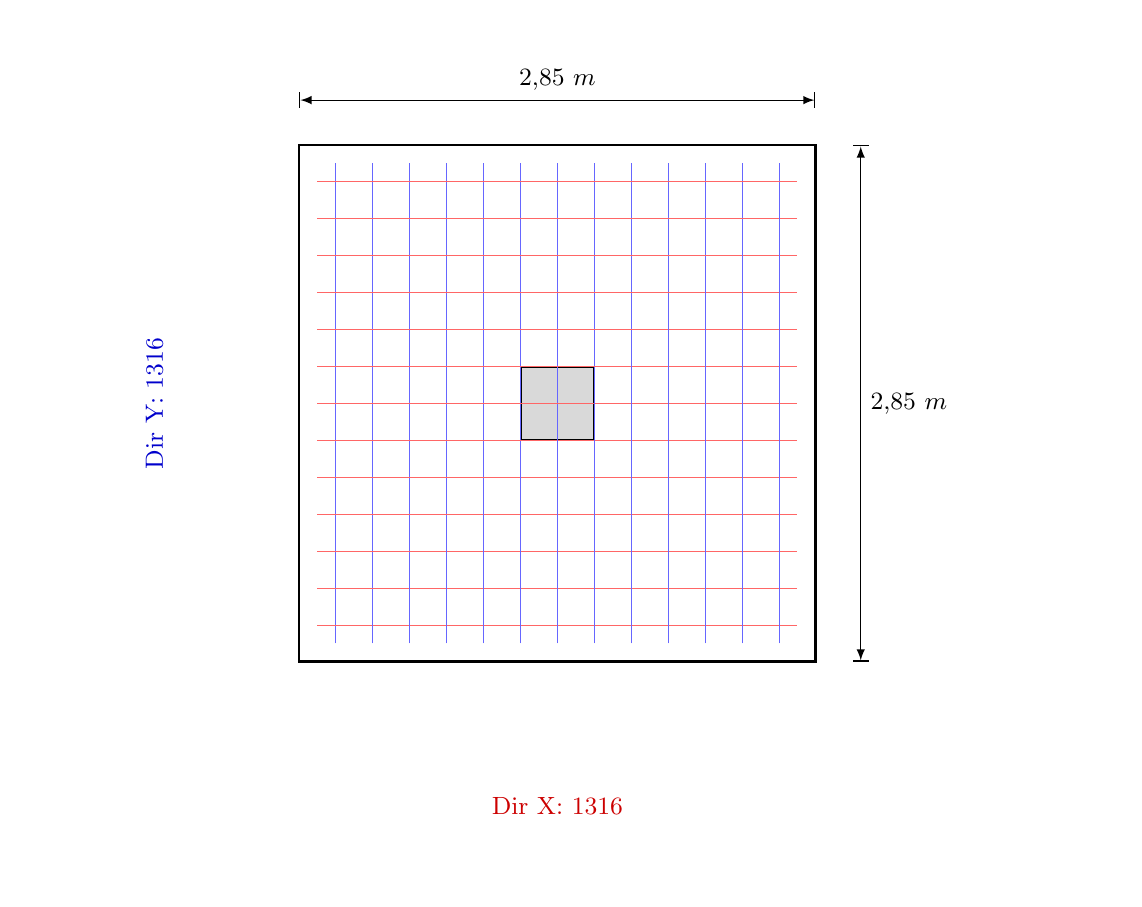
\begin{tikzpicture}[>=latex, scale=2.3]
        \path[use as bounding box] (-1.5, -1.2) rectangle (4.5, 3.5);
        \draw[thick] (0,0) rectangle (2.85, 2.85);
        \draw[thick, fill=gray!30] (1.225, 1.225) rectangle (1.625, 1.625);
        \foreach \x in {0.2, 0.404, 0.608, 0.812, 1.016, 1.22, 1.425, 1.63, 1.834, 2.038, 2.242, 2.446, 2.65} {
            \draw[blue!60, very thin] (\x, 0.1) -- (\x, 2.75);
            \draw[red!60, very thin] (0.1, \x) -- (2.75, \x);
        }
        \node[rotate=90, text=blue!80!black] at (-0.8, 1.425) {\small Dir Y: 13$\varnothing$16};
        \node[text=red!80!black] at (1.425, -0.8) {\small Dir X: 13$\varnothing$16};
        \draw[|<->|] (0, 3.1) -- (2.85, 3.1) node[midway, above] {\small $2{,}85\ \text{m}$};
        \draw[|<->|] (3.1, 0) -- (3.1, 2.85) node[midway, right] {\small $2{,}85\ \text{m}$};
    \end{tikzpicture}
    
    \vspace{0.2cm}
    \centerline{(a) Planta}
\end{figure}

%\newpage

\begin{figure}[H]
    \centering
    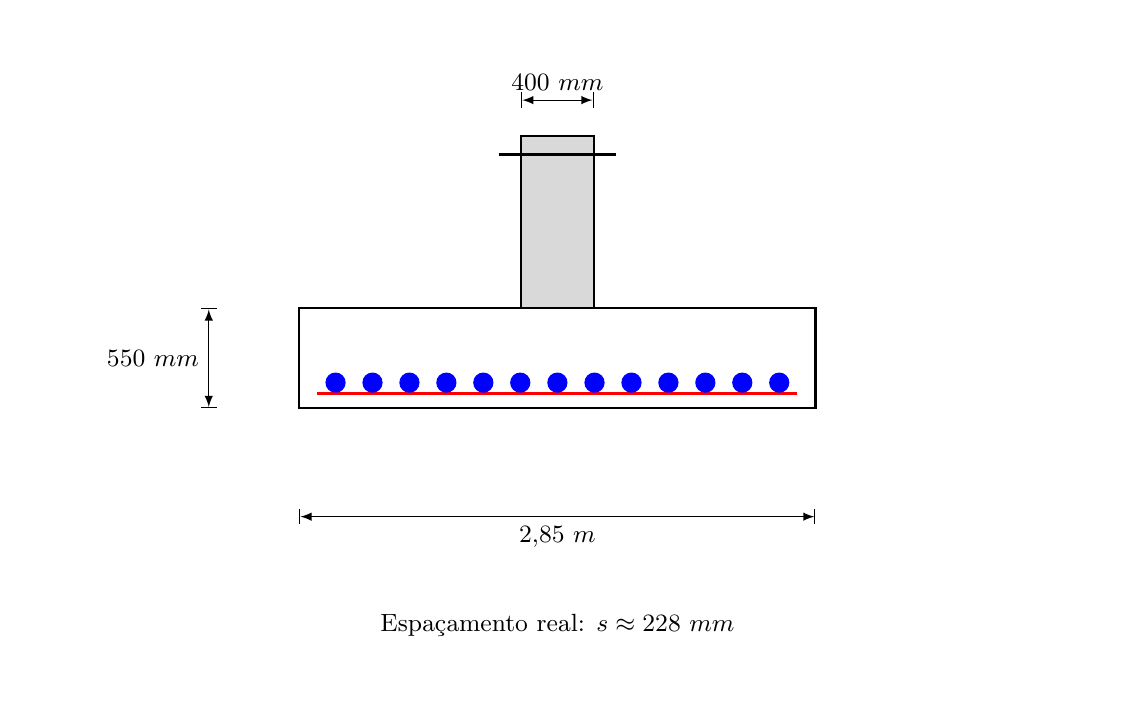
\begin{tikzpicture}[>=latex, scale=2.3]
        \path[use as bounding box] (-1.5, -1.6) rectangle (4.5, 2.1);
        \draw[thick] (0, 0) -- (2.85, 0) -- (2.85, 0.55) -- (0, 0.55) -- cycle;
        \draw[thick, fill=gray!30] (1.225, 0.55) rectangle (1.625, 1.5);
        \draw[thick] (1.1, 1.4) -- (1.75, 1.4); 
        \draw[thick, red] (0.1, 0.08) -- (2.75, 0.08);
        \foreach \x in {0.2, 0.404, 0.608, 0.812, 1.016, 1.22, 1.425, 1.63, 1.834, 2.038, 2.242, 2.446, 2.65} {
            \filldraw[blue] (\x, 0.14) circle (1.5pt);
        }
        \draw[|<->|] (-0.5, 0) -- (-0.5, 0.55) node[midway, left] {\small $550\ \text{mm}$};
        \draw[|<->|] (1.225, 1.7) -- (1.625, 1.7) node[midway, above] {\small $400\ \text{mm}$};
        \draw[|<->|] (0, -0.6) -- (2.85, -0.6) node[midway, below] {\small $2{,}85\ \text{m}$};
        \node at (1.425, -1.2) {\small Espaçamento real: $s \approx 228\ \text{mm}$};
    \end{tikzpicture}
    
    \vspace{0.2cm}
    \centerline{(b) Corte A-A}
    
    \vspace{0.6cm}
    \caption{Sapata dimensionada pela aplicação: (a) planta de armaduras e (b) corte transversal.}
    \label{fig:sapata_aplicacao}
\end{figure}

\begin{table}[H]
\centering
\caption{Comparação entre referência e a aplicação para a sapata isolada.}
\label{tab:comp_sapata}
\renewcommand{\arraystretch}{1.2}
\begin{tabular}{lcc}
\toprule
\textbf{Parâmetro} & \textbf{Mosley et al.} & \textbf{Aplicação} \\
\midrule
Dimensões \(A\times B\) [m] & \(2.80\times 2.80\) & \(2.85\times 2.85\) \\
Espessura \(H\) [m] & 0.60 & 0.55 \\
Área da base [m\(^2\)] & 7.84 & 8.12 \\
\(\sigma_{Ed}\) [kN/m\(^2\)] & 239.00 & 230.84 \\
Altura útil \(d\) [mm] & 520 & 480 \\
\(V_{Ed}\) punçoamento [kN] & 626 & 1034.67 \\
\(V_{Rd,c}\) [kN] & 1691 & 1078.97 \\
Armadura requerida & \(2243\ \text{mm}^2\) & \(9.07\ \text{cm}^2/\text{m}\) \\
Armadura adotada & \(12\phi16 @ 225\ \text{mm}\) & \(13\phi16\), \(s\approx 228\ \text{mm}\) \\
\bottomrule
\end{tabular}
\end{table}

\paragraph{Comparação dos resultados}

As duas soluções são estruturalmente coerentes e da mesma ordem de grandeza. A aplicação conduz a uma base ligeiramente maior em planta, mas a uma espessura total inferior, refletindo a natureza iterativa do algoritmo e a forma própria como este trata a verificação geotécnica, a estimativa do peso próprio e a procura do primeiro valor satisfatório de altura útil ao punçoamento. Apesar dessas diferenças, a solução final mantém margens de segurança adequadas e confirma a robustez do módulo desenvolvido.

\subsection{Conclusão da Validação}

A análise dos três casos de estudo confirma a consistência global da aplicação desenvolvida para o dimensionamento de vigas, pilares e sapatas isoladas segundo o Eurocódigo 2. Em todos os casos, os resultados obtidos revelaram concordância satisfatória com exemplos de referência da literatura, demonstrando que os algoritmos implementados reproduzem de forma coerente os principais procedimentos de cálculo, verificação e seleção construtiva da armadura.

No caso das vigas, a comparação com Goodchild et al. mostrou que a aplicação conduz a resultados muito próximos da resolução de referência, embora recorra a um procedimento mais rigoroso no recálculo da altura útil e do braço mecânico, com base na solução efetivamente adotada. Esta diferença metodológica traduz-se numa ligeira variação da área de armadura requerida, mas não compromete a coerência resistente nem a conformidade regulamentar da solução final.

Na validação do pilar, verificou-se igualmente boa concordância na definição geométrica, no comprimento eficaz e no cálculo da esbelteza. As diferenças observadas na classificação do elemento como esbelto ou não esbelto resultam essencialmente da adoção de parâmetros normativos distintos entre a referência bibliográfica e a aplicação, nomeadamente no valor de $\alpha_{cc}$ e no parâmetro $C$ da esbelteza limite. Assim, a divergência não decorre de erro de formulação, mas de opções explícitas de modelação normativa, sendo a resposta da aplicação coerente com os critérios implementados.

No caso da sapata isolada, a validação evidenciou a capacidade da aplicação para articular verificações geotécnicas e estruturais através de uma abordagem iterativa. Apesar de se observarem pequenas diferenças nas dimensões finais em planta, na espessura adotada e na discretização da armadura, a solução obtida manteve-se da mesma ordem de grandeza da solução bibliográfica e respeitou simultaneamente as verificações de tensão no solo, punçoamento e flexão. Este resultado confirma a robustez do algoritmo de dupla iteração e a sua adequação ao tipo de problema em estudo.

De forma transversal aos três módulos analisados, conclui-se que as diferenças residuais relativamente às referências não devem ser interpretadas como incongruências do sistema, mas antes como consequência de arredondamentos, critérios conservadores, diferentes anexos normativos, procedimentos iterativos mais rigorosos e discretização construtiva das armaduras. Neste sentido, a validação realizada permite afirmar que a aplicação constitui uma ferramenta tecnicamente credível, computacionalmente estável e metodologicamente coerente com os fundamentos teóricos e normativos adotados ao longo da dissertação.

Para além da comparação com a bibliografia, a incorporação de testes unitários automatizados reforça a fiabilidade do sistema, assegurando que alterações futuras ao código possam ser verificadas de forma objetiva e repetível. Assim, o processo de validação desenvolvido não só confirma a correção da implementação atual, como estabelece também uma base sólida para a evolução futura da aplicação, quer ao nível do alargamento a novos elementos estruturais, quer na integração com ferramentas complementares de análise e projeto.